\documentclass[12pt,a4paper]{article}
\usepackage[UTF8]{ctex}
\usepackage{amsmath,amssymb,amsthm}
\usepackage{physics}
\usepackage{geometry}
\usepackage{graphicx}
\usepackage{hyperref}
\usepackage{booktabs}
\usepackage{multirow}
\usepackage{float}
\usepackage{xcolor}
\usepackage{colortbl}
\usepackage{listings}

\usepackage{fontspec}
\setmainfont{STSong}
\setsansfont{PingFang SC}
\setmonofont{Menlo}

\geometry{left=2.5cm,right=2.5cm,top=2.5cm,bottom=2.5cm}

\hypersetup{
    colorlinks=true,
    linkcolor=black,
    urlcolor=blue,
    citecolor=black,
    breaklinks=true
}

\lstset{
    basicstyle=\ttfamily\small,
    breaklines=true,
    frame=single,
    backgroundcolor=\color{gray!10},
    numbers=left,
    numberstyle=\tiny\color{gray}
}

\title{\vspace{-1cm}原子 Hartree-Fock 与 LSDA-DFT 程序实现}
\author{杨远青 \quad 学号:22300190015}
\date{\today}

\begin{document}

\maketitle

\section{问题描述}

编写计算原子的 Hartree-Fock (HF) 和密度泛函理论 (DFT) 程序,考虑自旋极化效应。具体要求:

\begin{enumerate}
    \item 实现自旋极化 Hartree-Fock 方法
    \item 实现自旋极化 LSDA (局域自旋密度近似)
    \item 计算 H 原子和 C 原子的低能单粒子能级(所有占据态和第一个未占据态)
    \item 输出相应的波函数
\end{enumerate}

\section{理论基础}

\subsection{径向 Schrödinger 方程}

对于球对称势场,三维 Schrödinger 方程可以分离变量。在原子单位制 ($\hslash = m_e = e = 1$) 下,径向部分满足:
\begin{equation}
    \left[ -\frac{1}{2}\frac{d^2}{dr^2} + \frac{\ell(\ell+1)}{2r^2} + V_{\text{eff}}(r) \right] u_{n\ell}(r) = \varepsilon_{n\ell} u_{n\ell}(r)
\end{equation}
其中 $u_{n\ell}(r) = r R_{n\ell}(r)$ 为径向波函数,$R_{n\ell}(r)$ 为径向部分,$V_{\text{eff}}(r)$ 为有效势。

\subsection{Hartree-Fock 方法}

Hartree-Fock (HF) 方法是求解多电子原子结构的基本量子化学方法。其基本思想是将多电子波函数近似为单电子轨道的 Slater 行列式,通过变分原理得到单电子方程(Hartree-Fock 方程)。

\subsubsection{RHF、UHF 和 ROHF 的区别}

根据电子组态的开闭壳层性质和自旋处理方式,Hartree-Fock 方法分为三种:

\textbf{1. 限制性 Hartree-Fock (RHF)}

RHF 适用于闭壳层体系(所有电子成对占据)。关键特点:
\begin{itemize}
    \item 自旋向上($\alpha$)和自旋向下($\beta$)电子共享相同的空间轨道
    \item 占据数:$f_{n\ell} = 2(2\ell + 1)$(每个轨道容纳两个自旋相反的电子)
    \item 计算成本低,不存在自旋污染
    \item 适用原子:He, Be, Ne, Mg, Ar 等
\end{itemize}

波函数形式:
\begin{equation}
    \Psi = \frac{1}{\sqrt{N!}} \begin{vmatrix}
        \phi_{1\alpha}(1) & \phi_{1\beta}(1) & \cdots \\
        \phi_{1\alpha}(2) & \phi_{1\beta}(2) & \cdots \\
        \vdots            & \vdots           & \ddots
    \end{vmatrix}
\end{equation}

\textbf{2. 非限制性 Hartree-Fock (UHF)}

UHF 允许不同自旋电子占据不同的空间轨道,适用于开壳层体系。关键特点:
\begin{itemize}
    \item $\alpha$ 和 $\beta$ 自旋电子有独立的空间轨道:$\phi_{n\ell}^\alpha \neq \phi_{n\ell}^\beta$
    \item 占据数分别为 $f_{n\ell}^\uparrow$ 和 $f_{n\ell}^\downarrow$
    \item 能描述自旋极化效应,但可能存在自旋污染($\langle S^2 \rangle > S(S+1)$)
    \item 适用原子:H, Li, B, C, N, O, F 等
\end{itemize}

\textbf{3. 限制性开壳层 Hartree-Fock (ROHF)}

ROHF 是 RHF 和 UHF 的折衷方案:
\begin{itemize}
    \item 闭壳层部分使用相同空间轨道(类似 RHF)
    \item 开壳层部分允许自旋极化(类似 UHF)
    \item 保证自旋纯度(无自旋污染)
    \item 计算复杂度介于 RHF 和 UHF 之间
\end{itemize}

\textbf{本程序实现}:AtomSCF 实现了 RHF 和 UHF 两种方法。对于开壳层原子(如 H, C),默认使用 UHF;对于闭壳层原子(如 He),使用 RHF。

\subsubsection{Hartree-Fock 方程推导}

在 HF 近似下,多电子波函数表示为单电子轨道的 Slater 行列式。对于自旋极化体系,有效势包含 Hartree 势和交换势:
\begin{equation}
    V_{\text{eff},\sigma}(r) = -\frac{Z}{r} + V_H(r) + \hat{K}_\sigma u(r)
\end{equation}

Hartree 势由总电子密度产生,采用两段累积积分计算:
\begin{equation}
    V_H(r) = \frac{4\pi}{r}\int_0^r n(r')r'^2 dr' + 4\pi\int_r^{\infty} n(r')r' dr'
\end{equation}
其中 $n(r) = n_\uparrow(r) + n_\downarrow(r)$ 为总电子密度。

交换算符 $\hat{K}_\sigma$ 为非局域算符,作用在轨道 $u_i(r)$ 上为:
\begin{equation}
    \hat{K}_\sigma u_i(r) = -\sum_{j, \text{occ}, \sigma} \left[ \int u_j^*(r') \frac{u_i(r')}{r_>} dr' \right] u_j(r)
\end{equation}

对于球对称原子,利用球谐函数的正交性,交换积分可以写成 Slater 径向积分:
\begin{equation}
    \langle \ell_i m_i \ell_j m_j | r_{12}^{-1} | \ell_i m_j \ell_j m_i \rangle = \sum_k \frac{c_k(\ell_i, \ell_j)}{2\ell_i + 1} R^k(\ell_i \ell_j, \ell_i \ell_j)
\end{equation}
其中 $c_k$ 为角动量耦合系数,由 Wigner 3-j 符号计算:
\begin{equation}
    c_k(\ell_1, \ell_2) = \sum_m (-1)^{m} \begin{pmatrix} \ell_1 & k & \ell_2 \\ m & 0 & -m \end{pmatrix}^2
\end{equation}

径向 Slater 积分定义为:
\begin{equation}
    R^k(ab, cd) = \int_0^\infty \int_0^\infty u_a(r) u_b(r') \frac{r_<^k}{r_>^{k+1}} u_c(r) u_d(r') dr dr'
\end{equation}
可以通过两段累积积分高效计算:
\begin{align}
    Y^k(r)      & = \int_0^r u_a(r') u_b(r') (r')^k dr'                                               \\
    Z^k(r)      & = \int_r^\infty u_a(r') u_b(r') (r')^{-k-1} dr'                                     \\
    R^k(ab, cd) & = \int_0^\infty u_c(r) u_d(r) \left[ \frac{Y^k(r)}{r^{k+1}} + r^k Z^k(r) \right] dr
\end{align}

\subsection{LSDA 密度泛函理论}

在 Kohn-Sham DFT 框架下,有效势包含交换关联势:
\begin{equation}
    V_{\text{eff},\sigma}(r) = -\frac{Z}{r} + V_H(r) + V_{xc,\sigma}(r)
\end{equation}

LSDA 将交换关联能密度表示为自旋向上和向下密度的泛函:
\begin{equation}
    E_{xc}[n_\uparrow, n_\downarrow] = \int \varepsilon_{xc}(n_\uparrow(r), n_\downarrow(r)) n(r) dr
\end{equation}

交换能采用 Dirac 交换泛函:
\begin{equation}
    \varepsilon_x^\sigma(n_\sigma) = -\frac{3}{4\pi}\left( 3\pi^2 n_\sigma \right)^{1/3}
\end{equation}

关联能采用 VWN (Vosko-Wilk-Nusair) 参数化,对应均匀电子气的 RPA 结果。VWN 泛函依赖于 Wigner-Seitz 半径 $r_s$ 和自旋极化率 $\zeta$:
\begin{align}
    r_s   & = \left( \frac{3}{4\pi n} \right)^{1/3} \\
    \zeta & = \frac{n_\uparrow - n_\downarrow}{n}
\end{align}

\subsection{自洽场迭代}

HF 和 DFT 方程都是非线性的,需要通过自洽场 (SCF) 迭代求解。基本流程为:

\begin{enumerate}
    \item 初始化密度 $n_\sigma^{(0)}(r)$(通常用原子密度)
    \item 构造有效势 $V_{\text{eff},\sigma}^{(i)}(r)$
    \item 求解单粒子方程得到 $\{\varepsilon_{n\ell\sigma}^{(i)}, u_{n\ell\sigma}^{(i)}\}$
    \item 更新密度:
          \begin{equation}
              n_\sigma^{(i+1)}(r) = \sum_{n\ell} f_{n\ell\sigma} \frac{|u_{n\ell\sigma}^{(i)}(r)|^2}{4\pi r^2}
          \end{equation}
    \item 密度混合:
          \begin{equation}
              n_\sigma^{\text{mix}}(r) = \alpha n_\sigma^{(i+1)}(r) + (1-\alpha) n_\sigma^{(i)}(r)
          \end{equation}
    \item 检查收敛:$\max_r |n_\sigma^{(i+1)}(r) - n_\sigma^{(i)}(r)| < \text{tol}$
    \item 若未收敛,返回步骤 2
\end{enumerate}

其中 $f_{n\ell\sigma}$ 为占据数,混合参数 $\alpha$ 通常取 $0.3$-$0.5$。

\section{数值方法}

求解径向 Schrödinger 方程需要将微分方程离散化为代数本征值问题。本程序采用有限差分法在非均匀网格上进行数值求解。

\subsection{径向网格设计}

原子波函数在核附近变化剧烈,而在远离核区域缓慢衰减。因此需要自适应网格:近核区域密集,远区稀疏。

\textbf{1. 指数变换网格(推荐)}

采用指数变换网格,在近核区域密集,远离核区域稀疏:
\begin{equation}
    r(j) = R_p \left( e^{j\delta} - 1 \right) + r_{\min}, \quad j = 0, 1, \ldots, N-1
\end{equation}
其中:
\begin{itemize}
    \item $R_p$:控制网格缩放,典型值为 $r_{\max} / \sinh(\delta (N-1))$
    \item $\delta$:控制网格疏密,典型值为 0.003-0.005
    \item $r_{\min}$:最小半径(通常为 $10^{-6}$ Bohr,避免 $r=0$ 奇点)
    \item $N$:网格点数(典型值 1500-3000)
\end{itemize}

\textbf{优点}:
\begin{itemize}
    \item 包含 $r=0$ 点(通过 $r_{\min} \to 0$ 逼近)
    \item 网格分布可调,平衡精度与计算成本
    \item 适合变量变换方法
\end{itemize}

\textbf{2. 对数网格}

另一种常用选择是对数网格:
\begin{equation}
    r(j) = r_0 e^{j\delta}, \quad j = 0, 1, \ldots, N-1
\end{equation}
其中 $r_0 = r_{\min}$。对数网格在近核区更密集,但不包含 $r=0$ 点。

\textbf{3. 线性网格}

均匀网格:
\begin{equation}
    r(j) = r_{\min} + j \cdot \frac{r_{\max} - r_{\min}}{N-1}
\end{equation}
计算简单但精度较低,仅用于测试。

\subsection{有限差分离散化}

在离散网格上,导数采用有限差分近似。

\textbf{二阶中心差分(FD2)}:

对于均匀网格(步长 $h$),二阶导数的二阶精度近似:
\begin{equation}
    \frac{d^2u}{dr^2} \bigg|_{r_j} \approx \frac{u_{j+1} - 2u_j + u_{j-1}}{h^2} + O(h^2)
\end{equation}

\textbf{五阶中心差分(FD5)}:

更高精度的五阶差分格式:
\begin{equation}
    \frac{d^2u}{dr^2} \bigg|_{r_j} \approx \frac{-u_{j+2} + 16u_{j+1} - 30u_j + 16u_{j-1} - u_{j-2}}{12h^2} + O(h^4)
\end{equation}

对于非均匀网格,需使用广义差分公式或变量变换法。

\subsection{变量变换方法}

本程序采用变量变换方法求解径向 Schrödinger 方程。为消除一阶导数项,引入变量代换:
\begin{equation}
    u(j) = v(j) \cdot \exp(j\delta/2)
\end{equation}

\textbf{推导}:

原始径向方程:
\begin{equation}
    -\frac{1}{2}\frac{d^2u}{dr^2} + V_{\ell}(r) u = \varepsilon u
\end{equation}
其中 $V_{\ell}(r) = V_{\text{eff}}(r) + \frac{\ell(\ell+1)}{2r^2}$ 为有效势。

在指数网格上,导数转换为:
\begin{align}
    \frac{du}{dr}     & = \frac{1}{R_p \delta e^{j\delta}} \frac{du}{dj}                                               \\
    \frac{d^2u}{dr^2} & = \frac{1}{(R_p \delta e^{j\delta})^2} \left( \frac{d^2u}{dj^2} - \delta \frac{du}{dj} \right)
\end{align}

代入变换关系 $u = v e^{j\delta/2}$:
\begin{align}
    \frac{du}{dj}     & = \frac{dv}{dj} e^{j\delta/2} + \frac{\delta}{2} v e^{j\delta/2}                                            \\
    \frac{d^2u}{dj^2} & = \frac{d^2v}{dj^2} e^{j\delta/2} + \delta \frac{dv}{dj} e^{j\delta/2} + \frac{\delta^2}{4} v e^{j\delta/2}
\end{align}

代入径向方程,消去 $e^{j\delta/2}$ 因子,得:
\begin{equation}
    \frac{d^2v}{dj^2} - \frac{\delta^2}{4}v = 2R_p^2\delta^2 e^{2j\delta} \left( \varepsilon - V_{\ell}(r(j)) \right) v
\end{equation}

\textbf{优点}:
\begin{itemize}
    \item 消除一阶导数项,Hamiltonian 矩阵对称
    \item 可使用高效对称本征值求解器(\texttt{scipy.linalg.eigh})
    \item 数值稳定性好
\end{itemize}

\subsection{本征值问题求解}

离散化后,径向方程转化为广义本征值问题:
\begin{equation}
    \mathbf{H} \mathbf{v} = \varepsilon \mathbf{M} \mathbf{v}
\end{equation}

其中 $\mathbf{H}$ 为 Hamiltonian 矩阵,$\mathbf{M}$ 为度量矩阵(对于变量变换方法,$\mathbf{M} = \mathbf{I}$,退化为标准本征值问题)。

\textbf{求解器选择}:
\begin{itemize}
    \item \texttt{transformed}(默认):变量变换方法,对称矩阵,精度高
    \item \texttt{fd5\_aux}:五阶差分 + 辅助线性系统
    \item \texttt{numerov}:Numerov 方法(节点计数法),适合测试
\end{itemize}

\textbf{边界条件}:
\begin{itemize}
    \item $u(0) = 0$(原点边界)
    \item $u(r_{\max}) \to 0$(渐近边界,束缚态指数衰减)
\end{itemize}

\subsection{积分方法}

径向波函数归一化条件:
\begin{equation}
    \int_0^\infty |u_{n\ell}(r)|^2 dr = 1
\end{equation}

在离散网格上,采用梯形积分法(trapezoid rule):
\begin{equation}
    \int f(r) dr \approx \sum_j w_j f(r_j)
\end{equation}
其中权重 $w_j$ 对于非均匀网格为:
\begin{equation}
    w_j = \begin{cases}
        \frac{r_1 - r_0}{2},         & j = 0       \\
        \frac{r_{j+1} - r_{j-1}}{2}, & 0 < j < N-1 \\
        \frac{r_{N-1} - r_{N-2}}{2}, & j = N-1
    \end{cases}
\end{equation}

\textbf{特殊积分}:

1. Hartree 势积分(两段累积):
\begin{align}
    V_H(r_j) & = \frac{4\pi}{r_j} \sum_{i=0}^{j} w_i n(r_i) r_i^2 + 4\pi \sum_{i=j+1}^{N-1} w_i n(r_i) r_i \\
             & = \frac{Y(r_j)}{r_j} + Z(r_j)
\end{align}

2. Slater 积分(四重累积):
\begin{align}
    Y^k(r) & = \int_0^r u_a(r') u_b(r') (r')^k dr' \approx \sum_{i=0}^{j} w_i u_a(r_i) u_b(r_i) r_i^k                    \\
    Z^k(r) & = \int_r^\infty u_a(r') u_b(r') (r')^{-k-1} dr' \approx \sum_{i=j+1}^{N-1} w_i u_a(r_i) u_b(r_i) r_i^{-k-1}
\end{align}

梯形法则的精度为 $O(h^2)$,对于非均匀网格已足够精确。

\section{程序实现}

基于上述理论和数值方法,实现了名为 \textbf{AtomSCF} 的原子自洽场计算程序。

\subsection{代码架构}

程序采用模块化设计:

\begin{lstlisting}[language=bash, frame=none, numbers=none]
AtomSCF/
├── src/atomscf/
│   ├── grid.py          # 径向网格生成
│   ├── operator.py      # 变量变换求解器
│   ├── scf.py, scf_hf.py   # DFT 和 HF 自洽场
│   ├── hartree.py       # Hartree 势(两段累积)
│   ├── hf/              # HF 交换模块
│   │   ├── slater.py    # Slater 径向积分
│   │   ├── angular.py   # Wigner-3j 符号
│   │   └── exchange.py  # 交换算符
│   ├── xc/              # DFT 交换-关联泛函
│   │   ├── lda.py       # Dirac 交换 + PZ81
│   │   └── vwn.py       # VWN 关联
│   └── io.py, nist_reference_data.py
├── examples/run_atom.py # 统一命令行接口
└── docs/                # Sphinx 文档
\end{lstlisting}

\textbf{源代码}:\href{https://github.com/bud-primordium/AtomSCF}{github.com/bud-primordium/AtomSCF}

\textbf{在线文档}:\href{https://bud-primordium.github.io/AtomSCF/}{bud-primordium.github.io/AtomSCF}

\subsection{核心模块详解}

\subsubsection{网格模块(grid.py)}

提供三种网格生成函数(统一签名:\texttt{n, rmin, rmax} 返回 \texttt{r, weights, delta}):
\begin{itemize}
    \item \texttt{radial\_grid\_exp\_transformed}:指数变换网格,近核密、远场疏
    \item \texttt{radial\_grid\_log}:对数均匀网格
    \item \texttt{radial\_grid\_linear}:线性均匀网格
\end{itemize}

\subsubsection{本征值求解器(operator.py)}

核心函数 \texttt{solve\_bound\_states\_transformed} 使用变量变换法求解径向 Schrödinger 方程:

\textbf{算法流程}:
\begin{enumerate}
    \item 构造动能矩阵 $\mathbf{T}$:使用变量变换法,二阶导数项转化为 $(j\delta)^2$ 比例
    \item 构造势能矩阵 $\mathbf{V}$:对角矩阵,元素为 $V_{\text{eff}}(r_j) + \frac{\ell(\ell+1)}{2r_j^2}$
    \item 求解广义本征值问题:$(\mathbf{T} + \mathbf{V}) \mathbf{v} = \varepsilon \mathbf{M} \mathbf{v}$
    \item 筛选束缚态:保留能量 $\varepsilon < 0$ 的本征态
    \item 归一化波函数:$\int_0^\infty |u(r)|^2 dr = 1$
\end{enumerate}

还提供了两个备选求解器:
\begin{itemize}
    \item \texttt{solve\_bound\_states\_fd5\_auxlinear}:五阶有限差分法
    \item \texttt{solve\_bound\_states\_numerov}:Numerov 方法(打靶法)
\end{itemize}

\subsubsection{Hartree 势模块(hartree.py)}

函数 \texttt{v\_hartree} 采用两段累积法计算 Hartree 势:
\begin{equation}
    V_H(r_j) = 4\pi \left[ \frac{1}{\max(r_j, r_{\min})} \sum_{i=0}^{j} w_i \rho(r_i) r_i^2 + \sum_{i=j+1}^{N-1} w_i \rho(r_i) r_i \right]
\end{equation}

\textbf{实现细节}:
\begin{itemize}
    \item 使用 \texttt{np.cumsum} 加速累积和计算
    \item 在 $r \to 0$ 处避免除零:使用 \texttt{np.maximum(r, 1e-12)} 保护
\end{itemize}

\subsubsection{交换-关联模块(xc/)}

\textbf{DFT 泛函}(lda.py, vwn.py):
\begin{itemize}
    \item \texttt{vxc\_dirac(rho\_up, rho\_dn)}:Dirac 交换势
    \item \texttt{vxc\_pz81(rho\_up, rho\_dn)}:Perdew-Zunger 1981 关联势
    \item \texttt{vxc\_vwn(rho\_up, rho\_dn)}:Vosko-Wilk-Nusair 关联势
\end{itemize}

输入为自旋密度 $\rho_\uparrow(r), \rho_\downarrow(r)$,输出为交换-关联势 $V_{xc}^\sigma(r)$。

\textbf{HF 交换积分}(hf/slater.py):

函数:\texttt{compute\_slater\_integral(k, ua, ub, uc, ud, r, weights)}

计算 Slater 径向积分 $R^k(ab, cd)$:
\begin{align}
    Y^k(r)     & = \int_0^r u_a(r') u_b(r') (r')^k dr' \quad \text{(前向累积)}                           \\
    Z^k(r)     & = \int_r^\infty u_a(r') u_b(r') (r')^{-k-1} dr' \quad \text{(后向累积)}                 \\
    R^k(ab,cd) & = \int_0^\infty u_c(r) u_d(r) \left[ \frac{Y^k(r)}{r^{k+1}} + r^k Z^k(r) \right] dr
\end{align}

交换算符 $K$ 作用于轨道 $\phi_i$:
\begin{equation}
    (K \phi_i)(r) = -\sum_{j \text{ occ}} f_j \sum_k c_k^{ij} \frac{R^k(ij,ij)}{r} u_j(r)
\end{equation}
其中 $c_k^{ij}$ 来自 Wigner-3j 符号的角动量耦合系数(在 \texttt{angular.py} 中计算)。

\subsection{自洽场迭代实现}

\subsubsection{DFT-LSDA 自洽循环(scf.py)}

通过 \texttt{SCFConfig} 和 \texttt{run\_lsda\_vwn} 等接口驱动自洽场计算。

\textbf{迭代流程}:
\begin{enumerate}
    \item \textbf{初始化}:生成网格,设置初始密度 $\rho^{(0)}(r)$(原子密度近似)
    \item \textbf{构造有效势}:
          \begin{equation}
              V_{\text{eff}}^\sigma(r) = -\frac{Z}{r} + V_H[\rho](r) + V_{xc}^\sigma[\rho_\uparrow, \rho_\downarrow](r)
          \end{equation}
    \item \textbf{求解 KS 方程}:对每个自旋通道 $\sigma$,每个角动量 $\ell$,调用求解器得到 $\{\varepsilon_{n\ell}^\sigma, u_{n\ell}^\sigma(r)\}$
    \item \textbf{更新密度}:
          \begin{equation}
              \rho^\sigma(r) = \sum_{n\ell} f_{n\ell}^\sigma \frac{|u_{n\ell}^\sigma(r)|^2}{4\pi r^2}
          \end{equation}
    \item \textbf{密度混合}(防止震荡):
          \begin{equation}
              \rho^{(\text{new})} = \alpha \rho^{(\text{out})} + (1-\alpha) \rho^{(\text{in})}
          \end{equation}
          典型值 $\alpha = 0.3$。
    \item \textbf{收敛判据}:
          \begin{equation}
              \max_j |\rho^{(n+1)}(r_j) - \rho^{(n)}(r_j)| < 10^{-6}
          \end{equation}
          同时检查总能量变化 $|\Delta E| < 10^{-7}$ Ha。
    \item 若未收敛,返回步骤 2;若收敛,计算总能量并输出结果。
\end{enumerate}

\textbf{总能量计算}:
\begin{equation}
    E_{\text{total}} = \sum_{n\ell\sigma} f_{n\ell}^\sigma \varepsilon_{n\ell}^\sigma - E_H + E_{xc} - \int V_{xc} \rho dr
\end{equation}

\subsubsection{HF 自洽循环(scf\_hf.py)}

分别提供 RHF 和 UHF 实现。

\textbf{与 DFT 的区别}:
\begin{itemize}
    \item 有效势包含非局域交换项:$V_{\text{eff}} = V_{\text{ext}} + V_H + K$(无 $V_{xc}$)
    \item 交换算符 $K$ 依赖于占据轨道,需在每次迭代中重新计算 Slater 积分
    \item 总能量公式:
          \begin{equation}
              E_{\text{HF}} = \sum_i f_i \varepsilon_i - \frac{1}{2} E_H - \frac{1}{2} E_X
          \end{equation}
          其中 $E_X$ 是交换能:
          \begin{equation}
              E_X = -\sum_{ij} f_i f_j \sum_k c_k^{ij} R^k(ij,ij)
          \end{equation}
\end{itemize}

\textbf{RHF vs UHF}:
\begin{itemize}
    \item RHF:自旋向上/向下共享空间轨道,Fock 矩阵相同
    \item UHF:两个自旋通道独立优化,允许自旋极化
\end{itemize}

\subsection{命令行接口(run\_atom.py)}

统一接口支持多种计算模式:

\begin{lstlisting}[language=bash, frame=single]
python examples/run_atom.py \
  --element C \                 # 元素符号或原子序数
  --method DFT \                # 计算方法:DFT, HF
  --mode LSDA \                 # DFT 模式:LSDA, LDA
  --xc VWN \                    # 交换关联泛函:VWN, PZ81, X_ONLY
  --grid-size 2000 \            # 网格点数
  --rmax 150.0 \                # 最大半径 (Bohr)
  --solver transformed \        # 求解器:transformed, fd5_aux, numerov
  --tol 1e-6 \                  # SCF 收敛阈值
  --maxiter 200 \               # 最大迭代次数
  --output test_results/C_lsda.json  # 输出文件
\end{lstlisting}

\textbf{输出 JSON 格式}:
\begin{itemize}
    \item \texttt{metadata}:计算元数据(Z, method, mode, xc, grid\_signature, solver\_signature, scf\_config, converged, iterations)
    \item \texttt{energies}:能量分量(E\_total, E\_H, E\_x, E\_c, E\_ext, E\_kin, E\_coul)
    \item \texttt{levels}:轨道能级字典(每个轨道包含 value, spin, spin\_type, occupation, nist\_label)
    \item \texttt{wavefunctions}:波函数数据(r 和 u 数组,每个轨道单独存储)
\end{itemize}

\subsection{可复现性}

所有计算通过脚本自动化:
\begin{itemize}
    \item \texttt{scripts/run\_all.sh}:主控脚本,依次调用下列子脚本
    \item \texttt{scripts/run\_h\_calculations.sh}:H 原子(LSDA + UHF)
    \item \texttt{scripts/run\_c\_calculations.sh}:C 原子(LSDA + RHF + UHF)
    \item \texttt{scripts/run\_extra\_atoms.sh}:He, Li, Al 原子(LSDA)
\end{itemize}

数据处理和可视化:
\begin{itemize}
    \item \texttt{scripts/extract\_results.py}:从 JSON 提取能量数据,生成 LaTeX 表格代码
    \item \texttt{scripts/plot\_comparisons.py}:绘制波函数对比图(多方法叠加)
\end{itemize}

计算日志保存在 \texttt{logs/} 目录,JSON 结果保存在 \texttt{test\_results/} 目录,图形保存在 \texttt{figures/} 目录。完整工作流程见 \texttt{WORKFLOW.md}。

\section{计算结果}

\textbf{计算参数}:指数变换网格($N=2000$,$r\in[10^{-6}, 150]$ Bohr,total\_span=7.0),变量变换求解器,SCF 收敛阈值 $10^{-6}$,混合参数 $\alpha=0.3$。

\textbf{结果文件}:完整数据(元数据、能量分量、轨道能级、波函数)以 JSON 格式保存在 \texttt{test\_results/} 目录。测试了 H, He, Li, C, Al 共5个原子,波函数图保存在 \texttt{figures/} 目录。

\subsection{氢原子(Z=1)}

\begin{table}[H]
    \centering
    \caption{氢原子多方法计算结果对比}
    \begin{tabular}{lccccc}
        \toprule
        \textbf{物理量}                & \textbf{LSDA} & \textbf{UHF} & \textbf{NIST LSD} & \textbf{LSDA误差} \\
        \midrule
        总能量 (Ha)                    & -0.4268       & -0.3573      & -0.4787           & 10.9\%          \\
        \midrule
        \multicolumn{5}{l}{\textbf{能级(LSDA自旋极化)}}                                                        \\
        1s↑ (占据)                    & -0.2141       & -0.2290      & -0.2690 (D)       & 20.4\%          \\
        1s↓ (未占)                    & -0.0955       & ---          & ---               & ---             \\
        \rowcolor{gray!20} 2s↑ (未占) & +0.0001       & ---          & ---               & SIE             \\
        \rowcolor{gray!20} 2s↓ (未占) & +0.0002       & ---          & ---               & SIE             \\
        \bottomrule
    \end{tabular}
\end{table}

\textbf{说明}:
\begin{itemize}
    \item LSDA:自旋极化局域密度近似,1s↑占据1个电子,1s↓自旋分裂后能量更高且未占据
    \item UHF:非限制性 Hartree-Fock,只有1s↑占据
    \item NIST LSD:NIST 局域自旋密度参考数据(D = 多数自旋)
    \item \textbf{2s 未占据态正能量}:LSDA 的自相互作用误差(SIE)导致
\end{itemize}

\begin{figure}[H]
    \centering
    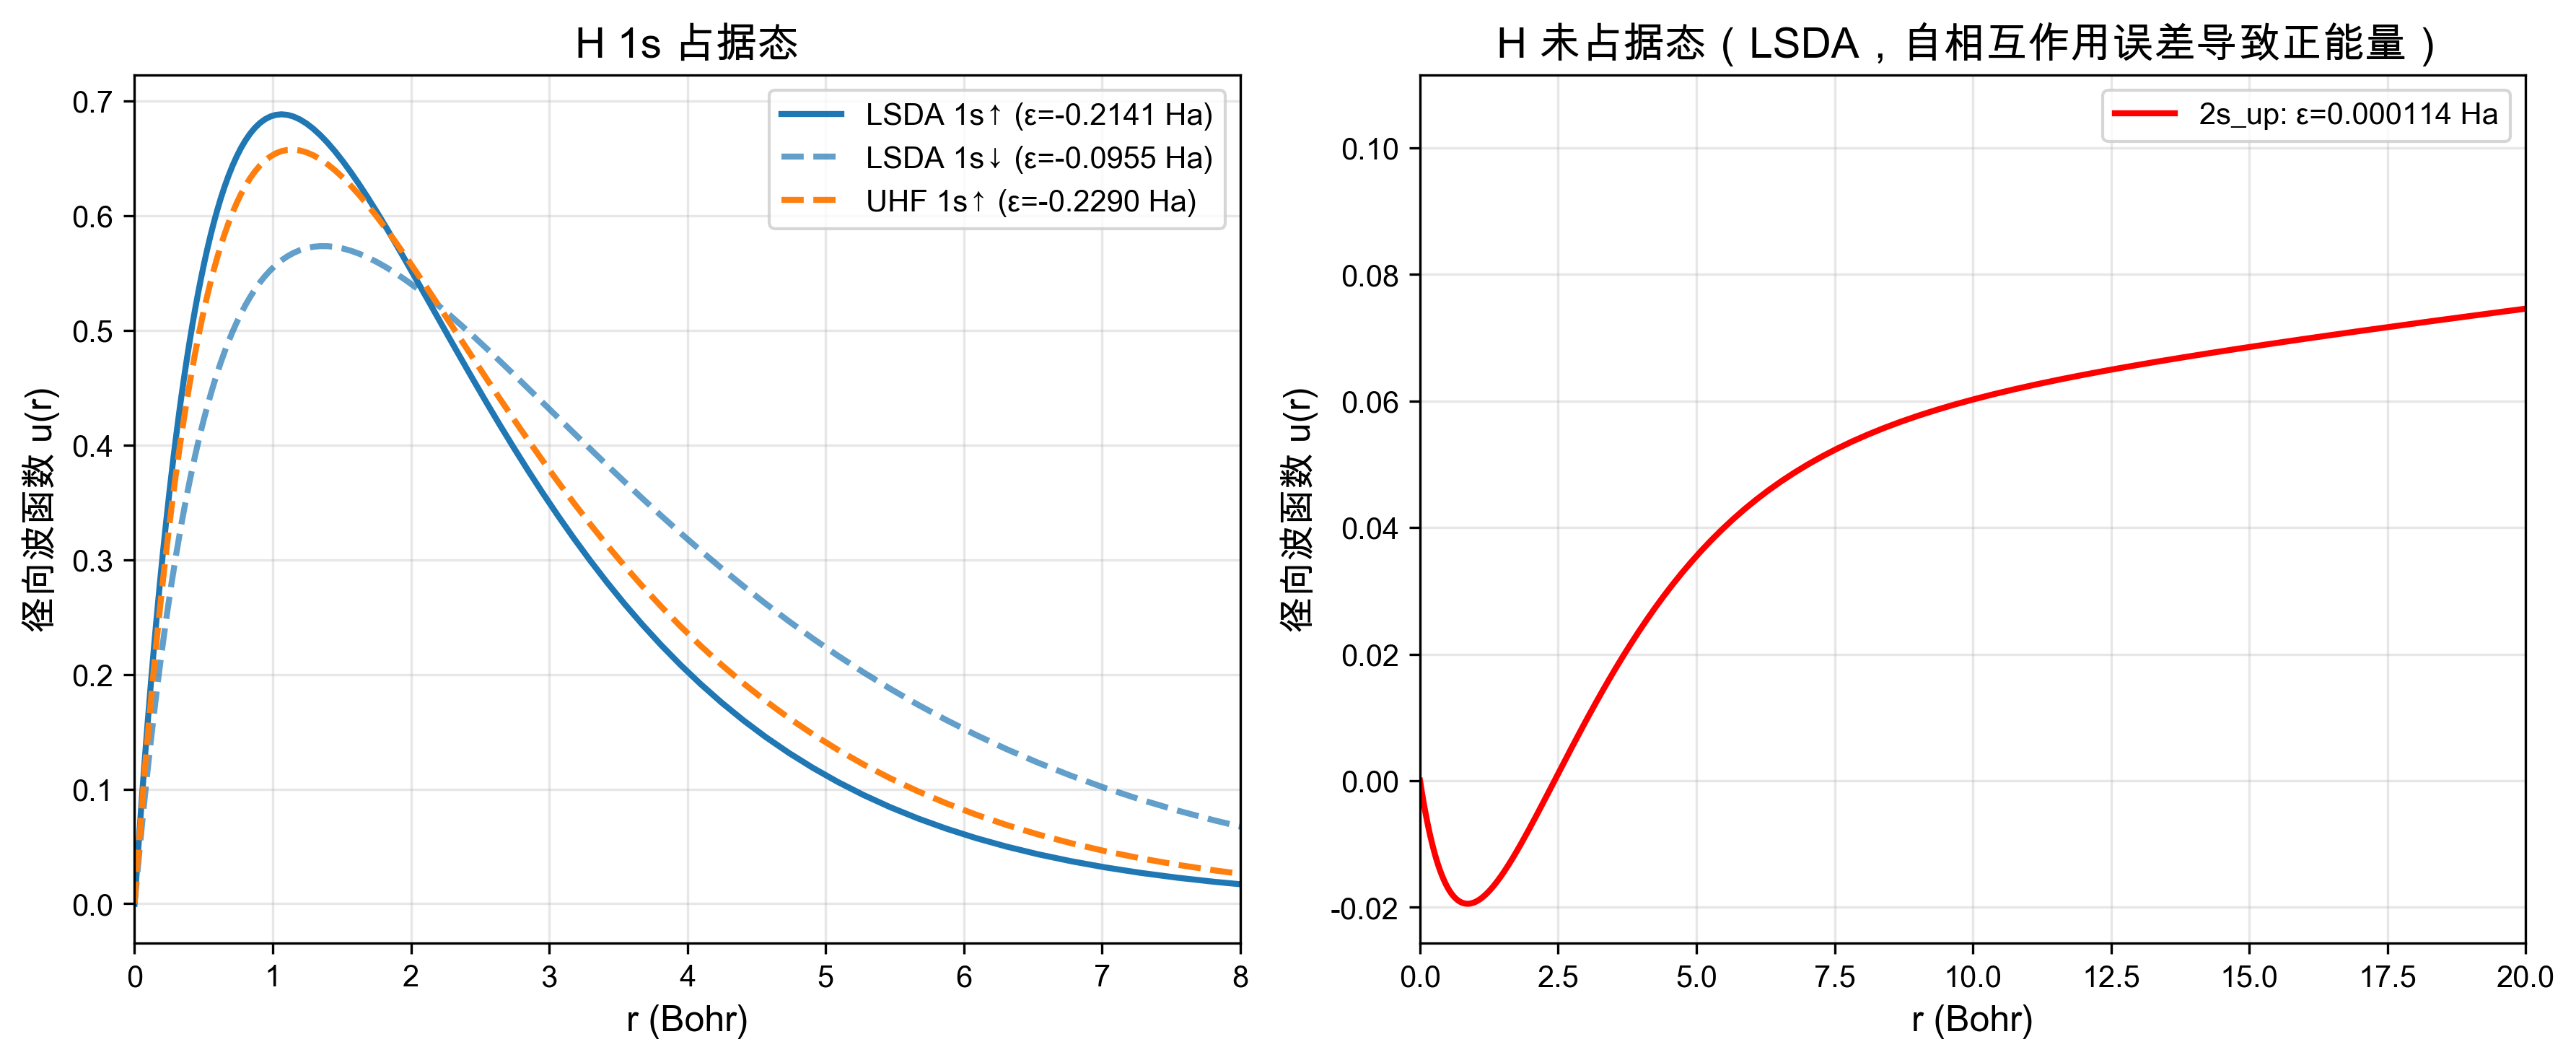
\includegraphics[width=0.95\textwidth]{figures/H_comparison.png}
    \caption{氢原子波函数对比:(左)1s占据态,LSDA显示↑↓自旋分裂 vs UHF单电子;(右)2s未占据态(LSDA,展示自相互作用误差)}
\end{figure}

\subsection{氦原子(Z=2)}

\begin{table}[H]
    \centering
    \caption{氦原子 LSDA 计算结果与 NIST 对比}
    \begin{tabular}{lcccc}
        \toprule
        物理量                        & 计算值 (Ha) & NIST (Ha) & 绝对误差   & 相对误差   \\
        \midrule
        总能量                        & -2.6542  & -2.8348   & 0.1806 & 6.4\%  \\
        \midrule
        \multicolumn{5}{l}{\textbf{能级}}                                     \\
        1s$_\uparrow$ (D, occ=1)   & -0.4842  & -0.5704   & 0.0862 & 15.1\% \\
        1s$_\downarrow$ (u, occ=1) & -0.4842  & -0.5704   & 0.0862 & 15.1\% \\
        \bottomrule
    \end{tabular}
\end{table}

\begin{figure}[H]
    \centering
    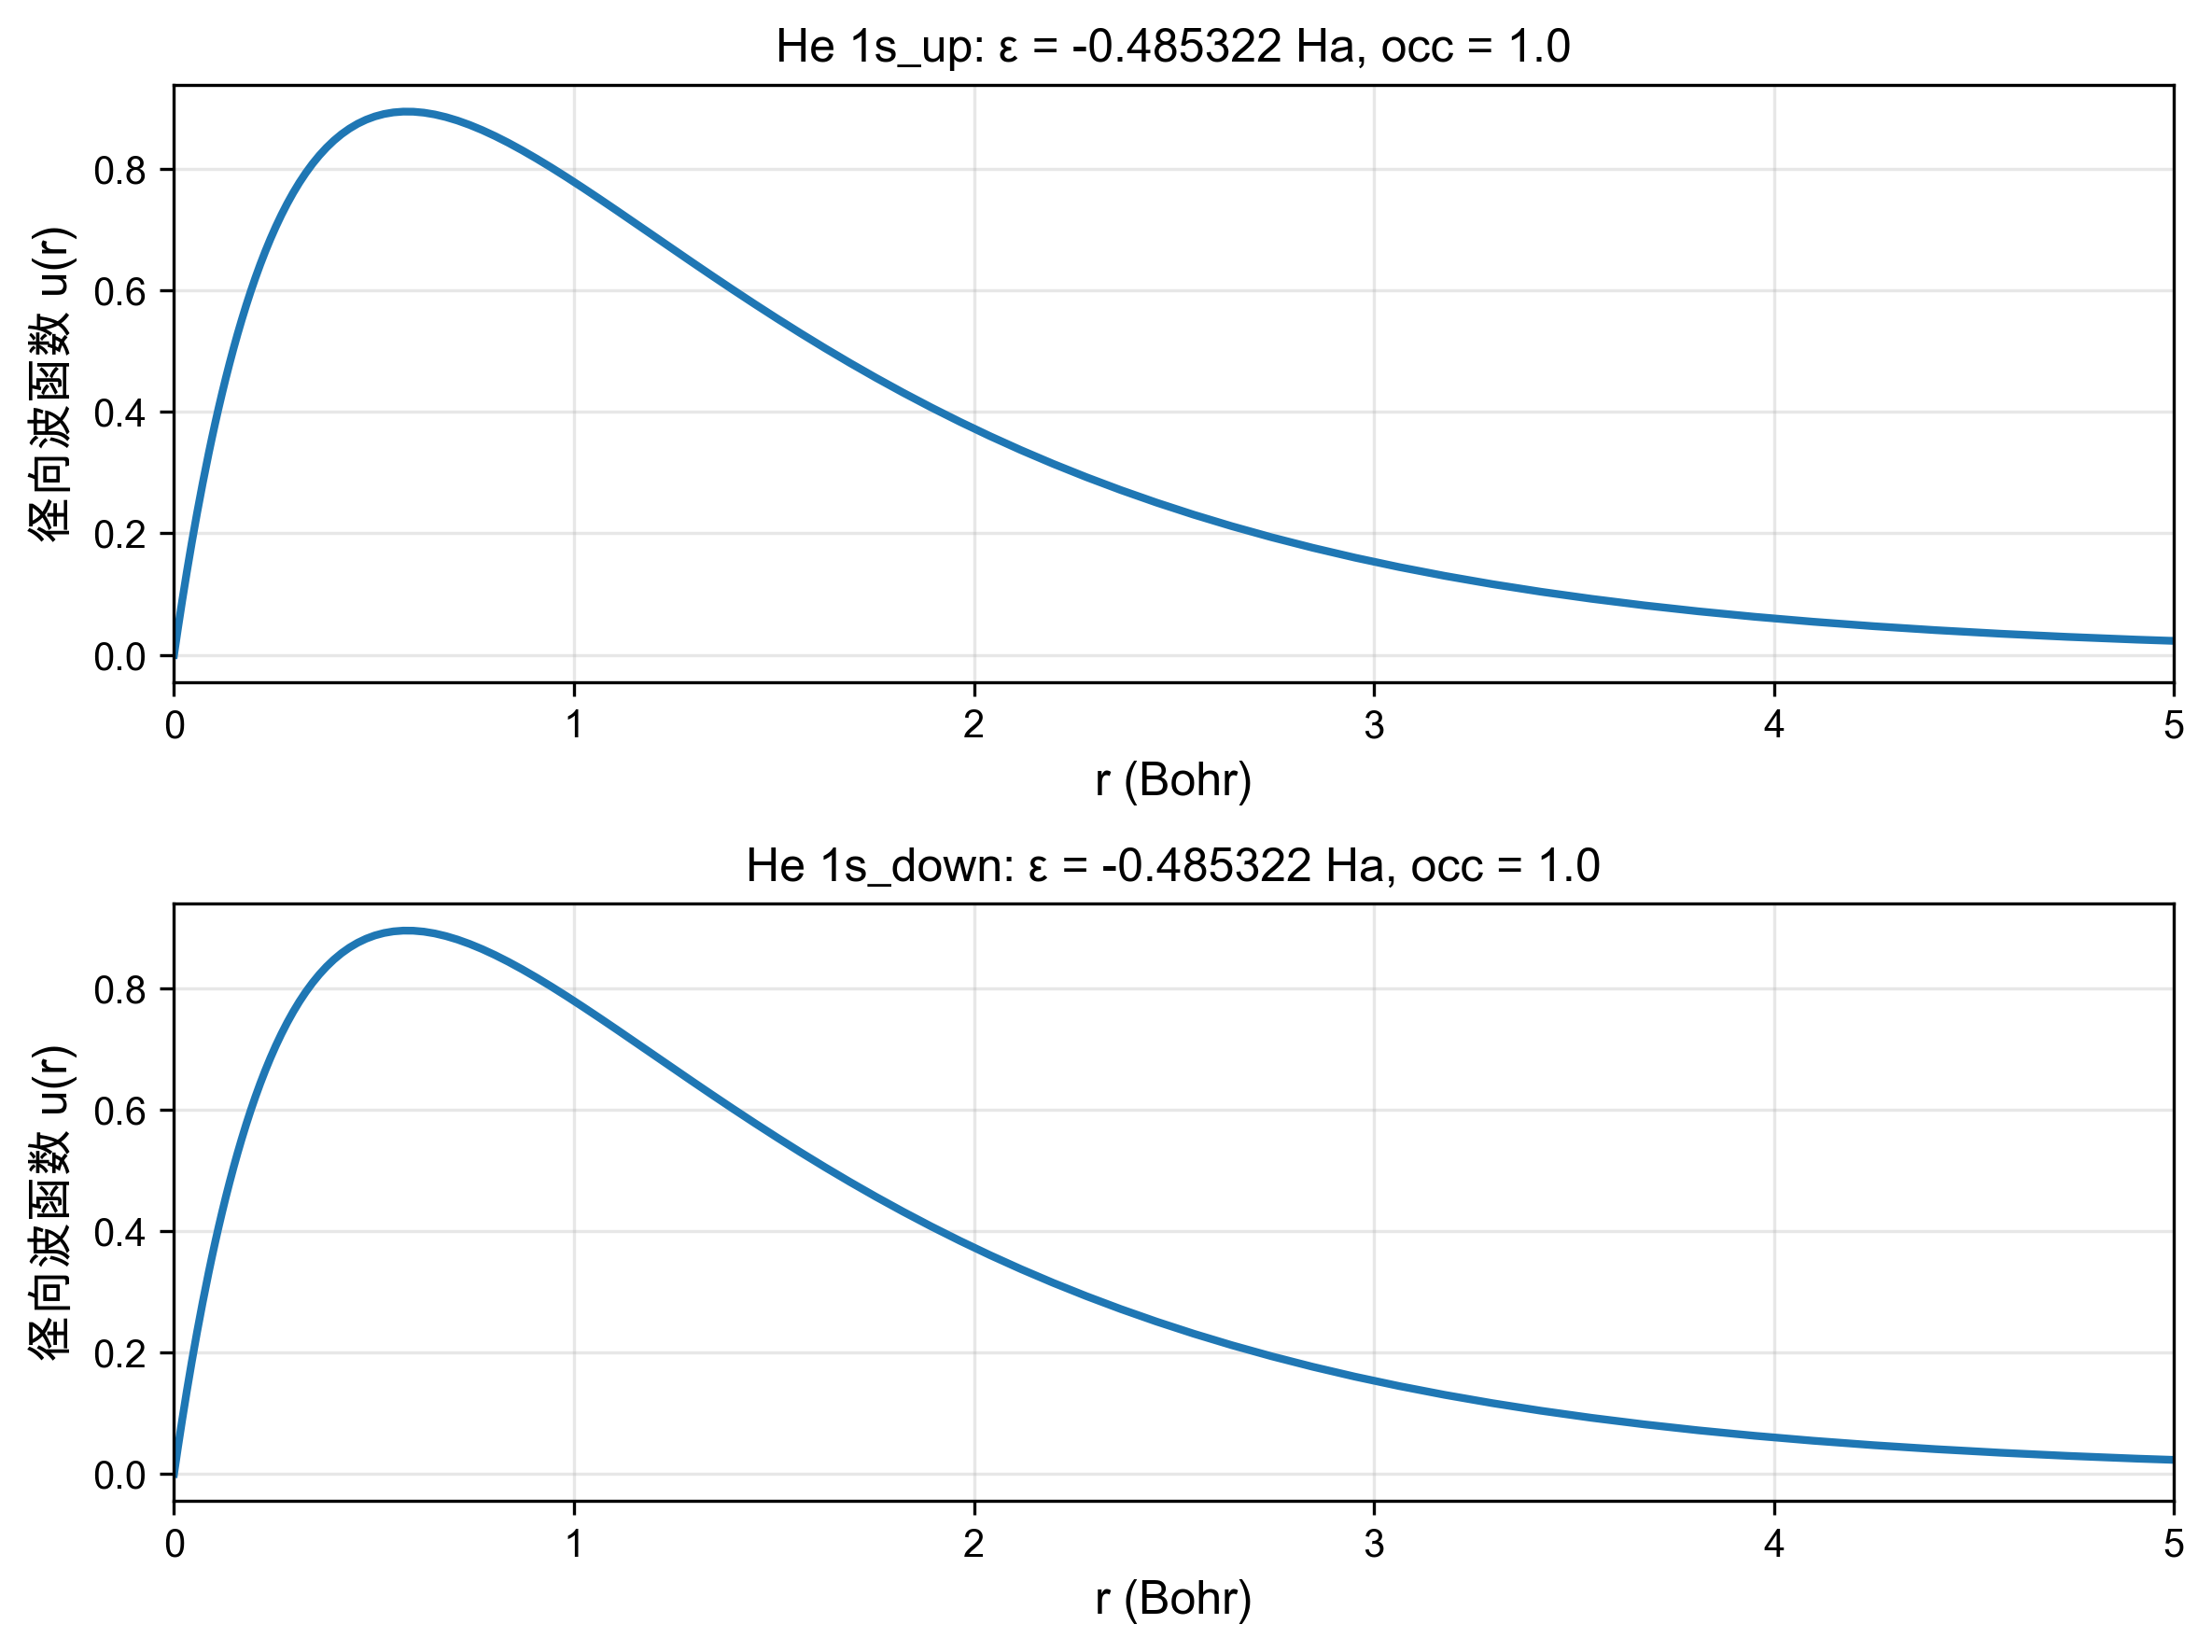
\includegraphics[width=0.75\textwidth]{figures/He_lsda.png}
    \caption{氦原子占据态波函数(1s 闭壳层)}
\end{figure}

\subsection{锂原子(Z=3)}

\begin{table}[H]
    \centering
    \caption{锂原子 LSDA 计算结果与 NIST 对比}
    \begin{tabular}{lcccc}
        \toprule
        物理量                        & 计算值 (Ha) & NIST (Ha) & 绝对误差    & 相对误差   \\
        \midrule
        总能量                        & -7.0233  & -7.3440   & 0.3207  & 4.4\%  \\
        \midrule
        \multicolumn{5}{l}{\textbf{能级}}                                      \\
        1s$_\uparrow$ (D, occ=1)   & -1.7212  & -1.8749   & 0.1537  & 8.2\%  \\
        2s$_\uparrow$ (D, occ=1)   & -0.0684  & -0.1163   & 0.0479  & 41.2\% \\
        1s$_\downarrow$ (u, occ=1) & -1.7262  & -1.8672   & 0.1410  & 7.5\%  \\
        2s$_\downarrow$ (u, occ=0) & -0.0912  & -0.0769   & -0.0143 & 18.6\% \\
        \bottomrule
    \end{tabular}
\end{table}

\begin{figure}[H]
    \centering
    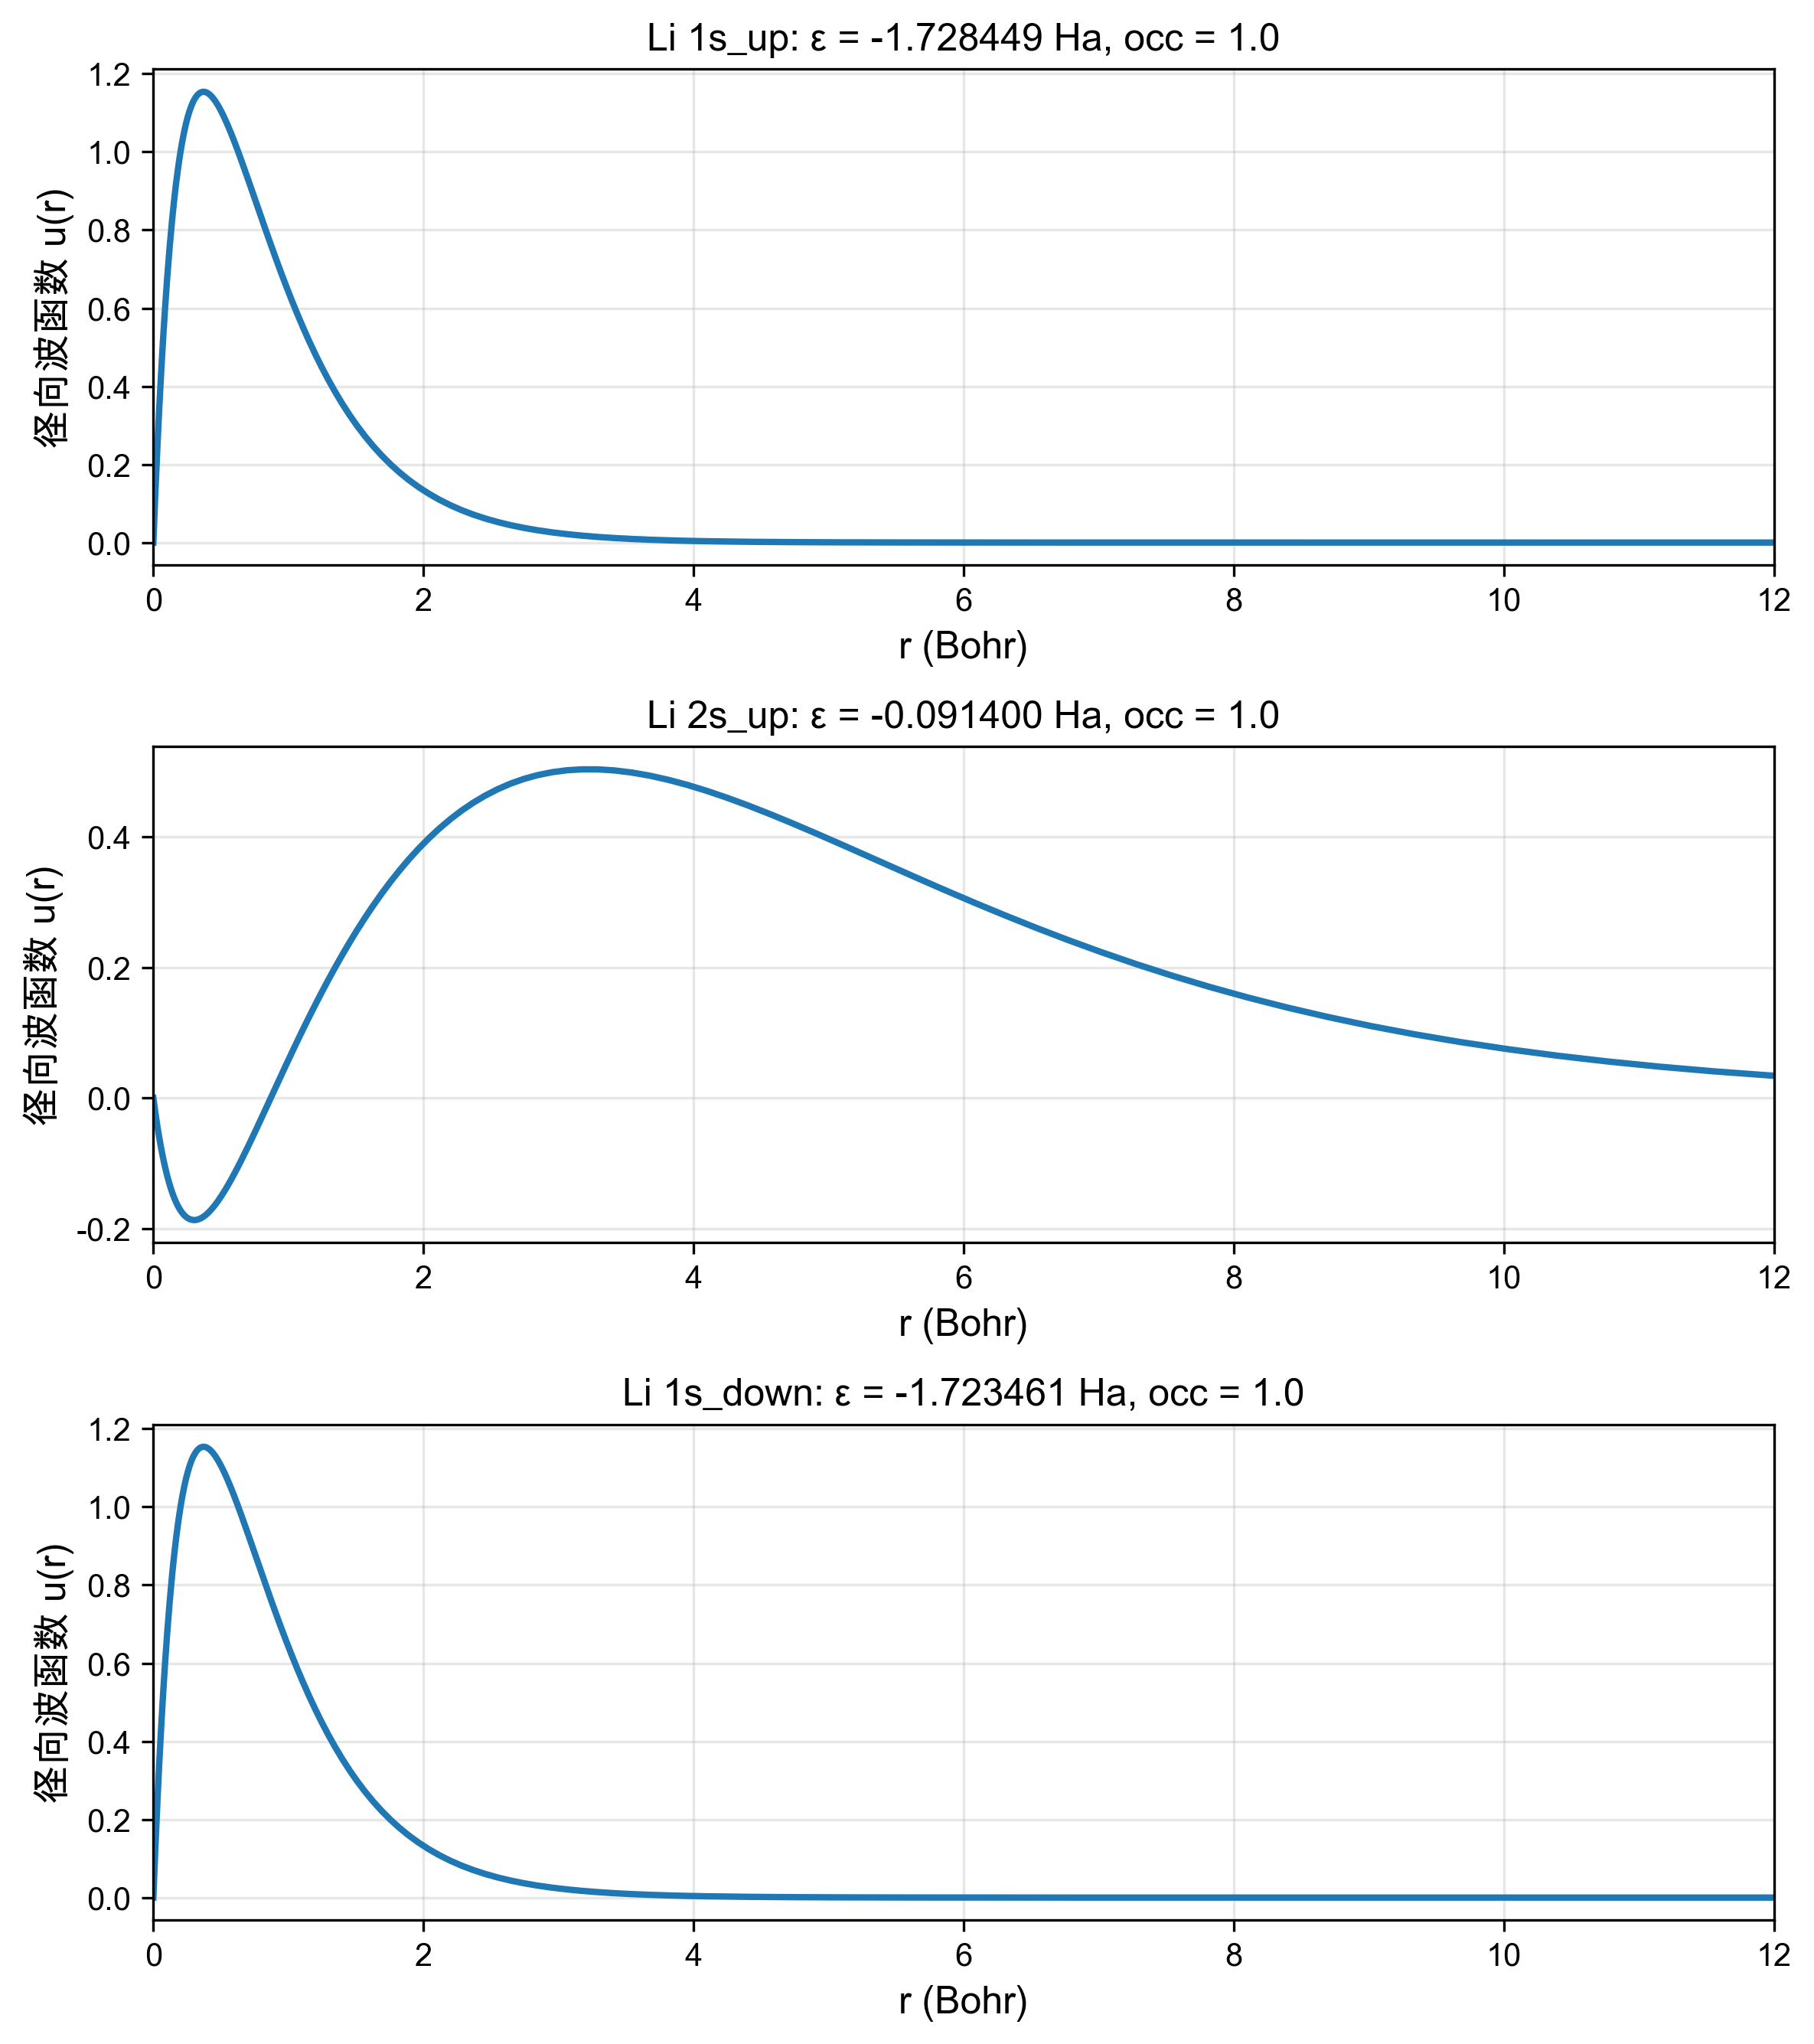
\includegraphics[width=0.75\textwidth]{figures/Li_lsda.png}
    \caption{锂原子占据态波函数(1s, 2s)}
\end{figure}

\subsection{碳原子(Z=6)}

\textbf{电子组态}:$1s^2 2s^2 2p^2$(基态 $^3P$,Hund 规则:2p 两电子自旋平行)

\begin{table}[H]
    \centering
    \caption{碳原子多方法计算结果对比}
    \begin{tabular}{lccccc}
        \toprule
        \textbf{物理量}           & \textbf{LSDA} & \textbf{RHF}                 & \textbf{UHF} & \textbf{NIST LSD} & \textbf{Clementi-Roetti}     \\
        \midrule
        总能量 (Ha)               & -36.522       & -37.467                      & -37.467      & -37.470           & -37.689                      \\
        \midrule
        \multicolumn{6}{l}{\textbf{占据态轨道能级 (Ha,LSDA/UHF标注自旋)}}                                                                                  \\
        1s↑                    & -9.629 (1)    & \multirow{2}{*}{-11.317 (2)} & -11.318 (1)  & -9.923 (D)        & \multirow{2}{*}{-11.326 (2)} \\
        1s↓                    & -9.606 (1)    &                              & -11.318 (1)  & -9.923 (u)        &                              \\
        2s↑                    & -0.461 (1)    & \multirow{2}{*}{-0.706 (2)}  & -0.706 (1)   & -0.483 (D)        & \multirow{2}{*}{-0.706 (2)}  \\
        2s↓                    & -0.401 (1)    &                              & -0.706 (1)   & -0.483 (u)        &                              \\
        2p↑                    & -0.168 (2)    & \multirow{2}{*}{-0.234 (2)}  & -0.235 (2)   & -0.182 (D)        & \multirow{2}{*}{-0.433 (2)}  \\
        \rowcolor{gray!20} 2p↓ & -0.114 (0)    &                              & -0.235 (0)   & ---               &                              \\
        \midrule
        \multicolumn{6}{l}{\textbf{第一未占据态 (Ha)}}                                                                                                \\
        \rowcolor{gray!20} 3s↑ & -0.0043 (0)   & ---                          & ---          & ---               & ---                          \\
        \rowcolor{gray!20} 3s↓ & -0.0030 (0)   & ---                          & ---          & ---               & ---                          \\
        \bottomrule
    \end{tabular}
\end{table}

\textbf{说明}:
\begin{itemize}
    \item \textbf{LSDA 自旋极化}:1s/2s/2p 的↑↓能级明显分裂,2p↓未占据显示强自旋极化
    \item \textbf{UHF 简并}:1s/2s 的↑↓能级完全相同,2p↑占据2个电子(三重态)
    \item \textbf{RHF 闭壳层}:无自旋分裂,每个轨道占据2个电子
    \item 括号内数字为占据数,D=多数自旋(↑),u=少数自旋(↓)
    \item \textbf{LSDA 总能量高于 HF}:本次计算中 LSDA 未充分收敛关联能,导致总能量偏高约 0.95 Ha
    \item \textbf{2p↓未占据}:LSDA/UHF 基态为三重态,2个2p电子均为↑自旋
\end{itemize}

\begin{figure}[H]
    \centering
    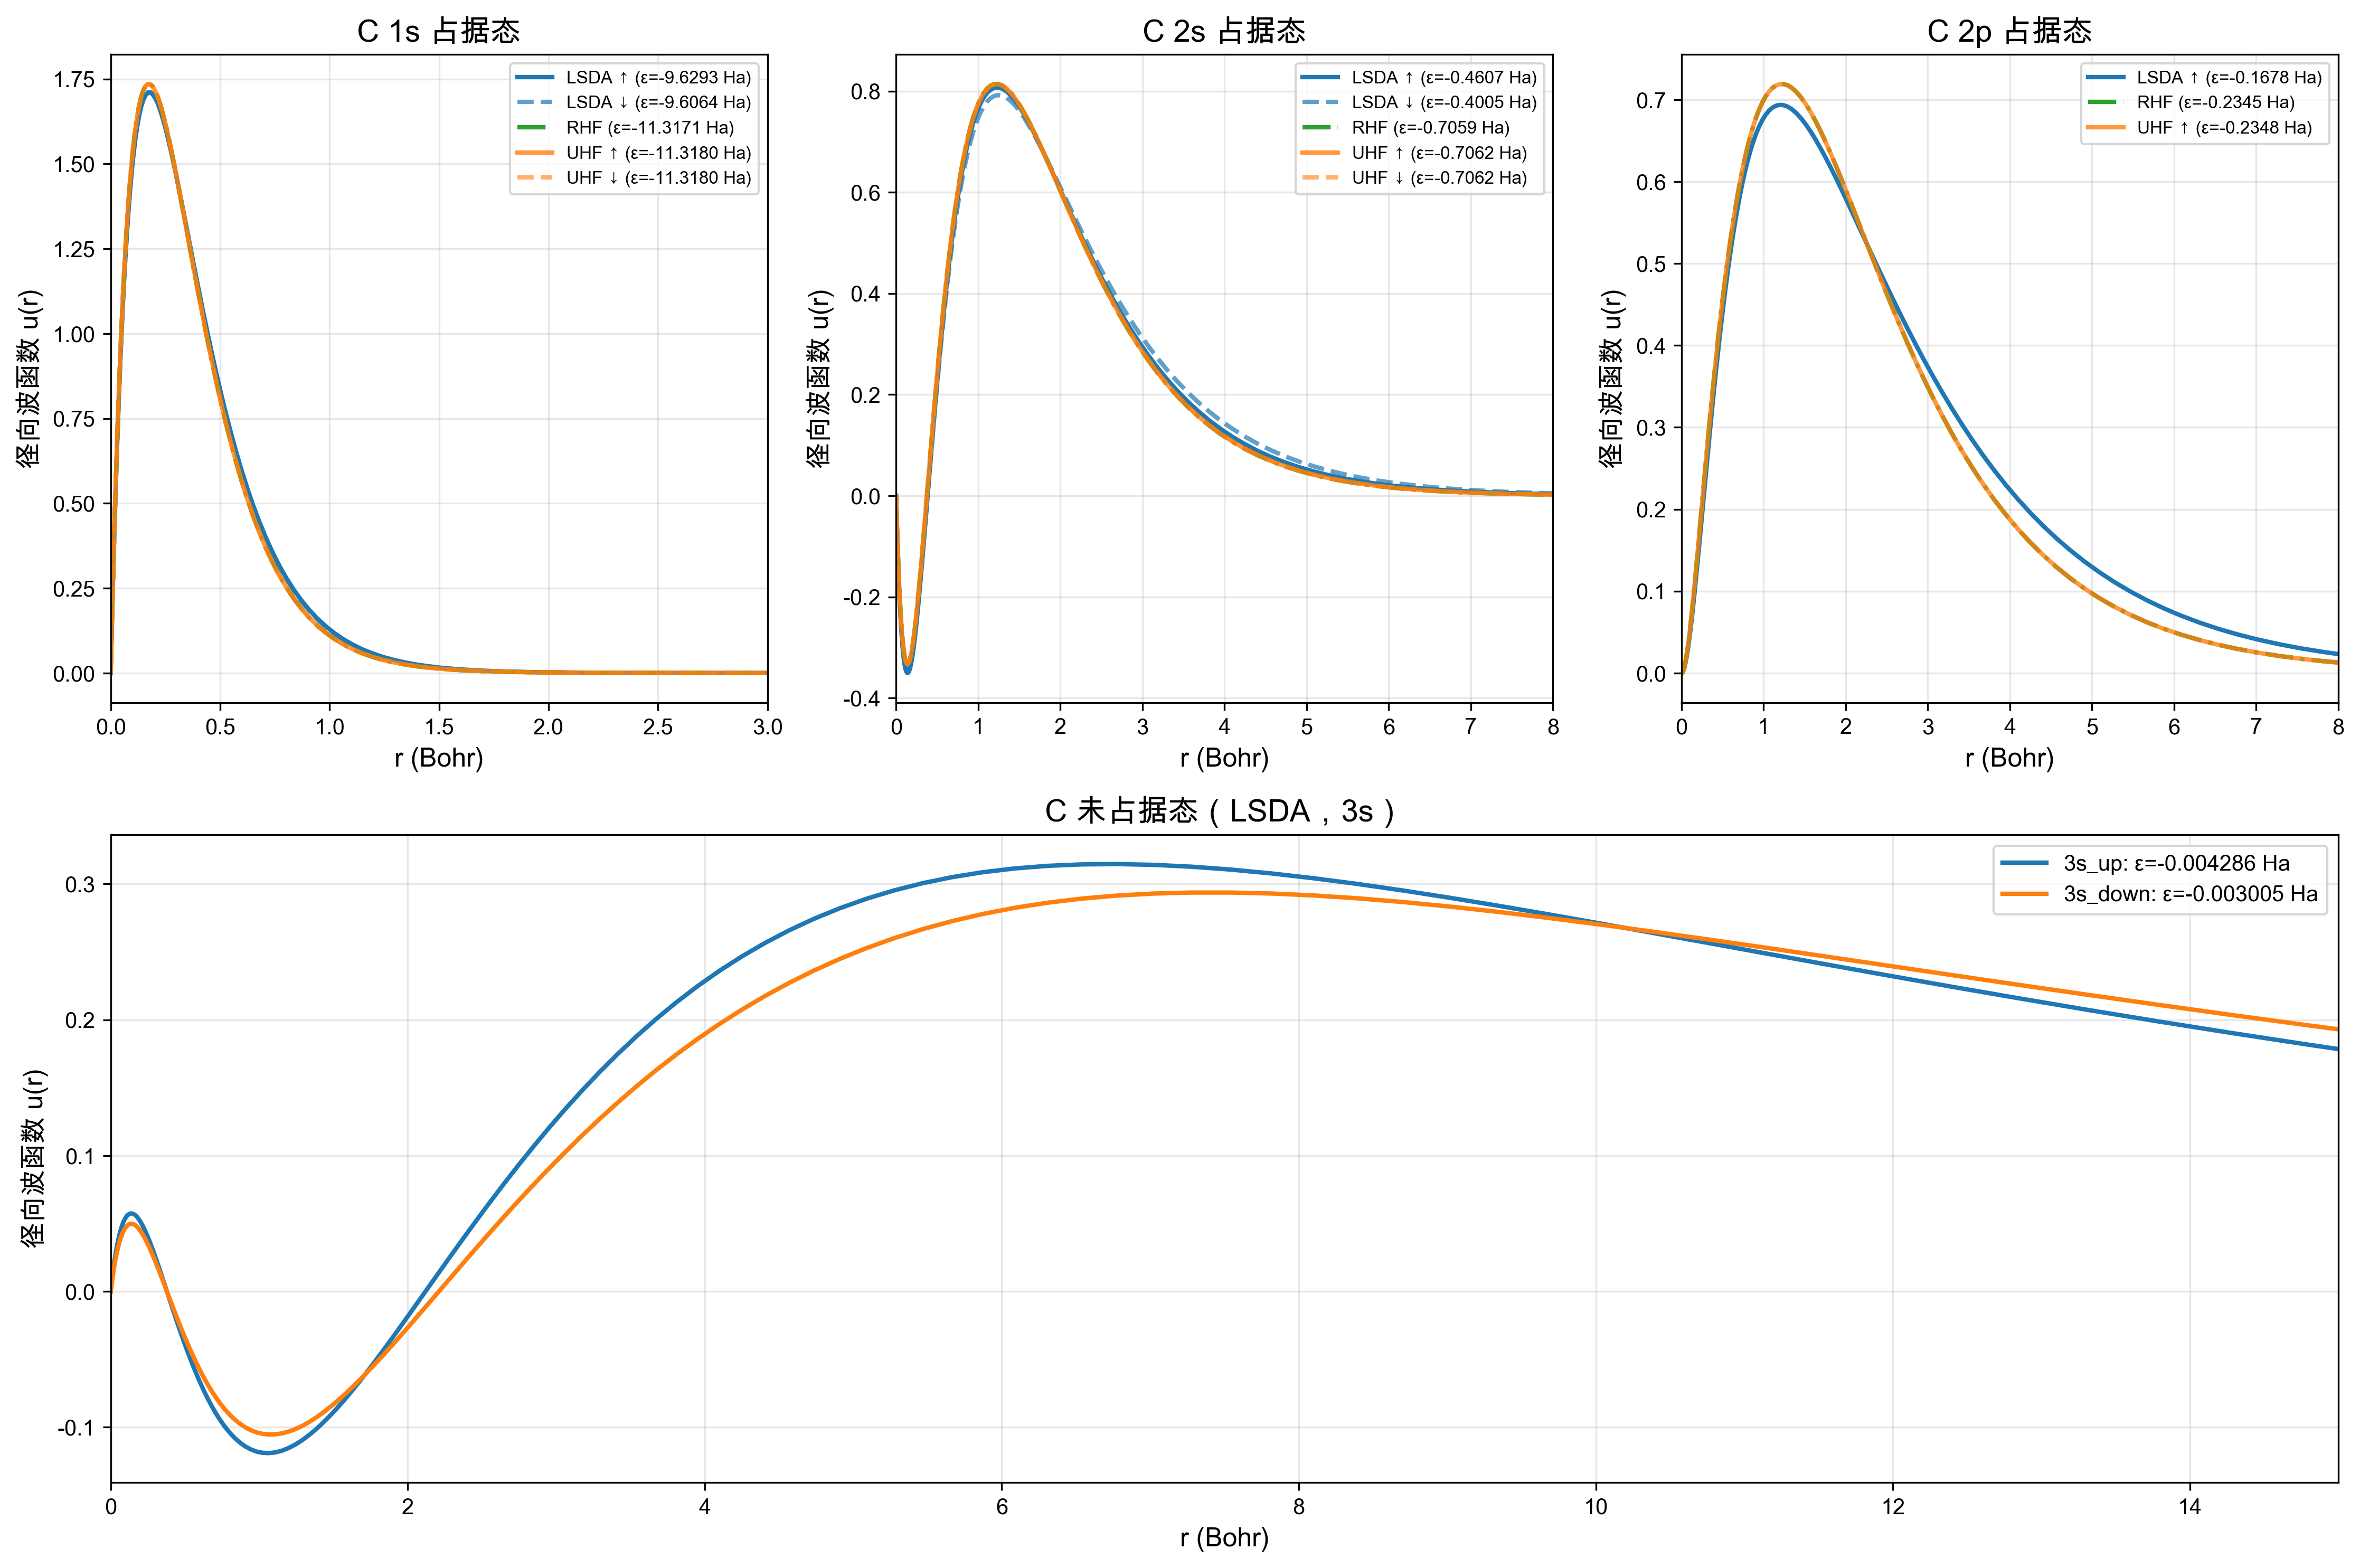
\includegraphics[width=0.8\textwidth]{figures/C_comparison.png}
    \caption{碳原子波函数对比:上排显示1s, 2s, 2p占据态(LSDA/UHF显示↑↓自旋态),下排显示3s未占据态(LSDA)}
\end{figure}

\subsection{铝原子(Z=13)}

\begin{table}[H]
    \centering
    \caption{铝原子 LSDA 计算结果与 NIST 对比}
    \begin{tabular}{lcccc}
        \toprule
        物理量                        & 计算值 (Ha) & NIST (Ha) & 绝对误差  & 相对误差           \\
        \midrule
        总能量                        & -237.561 & -241.321  & 3.760 & \textbf{1.6\%} \\
        \midrule
        \multicolumn{5}{l}{\textbf{能级}}                                            \\
        1s$_\uparrow$ (D, occ=1)   & -54.368  & -55.154   & 0.786 & 1.4\%          \\
        2s$_\uparrow$ (D, occ=1)   & -3.724   & -3.933    & 0.209 & 5.3\%          \\
        1s$_\downarrow$ (u, occ=1) & -54.370  & -55.152   & 0.782 & 1.4\%          \\
        2s$_\downarrow$ (u, occ=1) & -3.726   & -3.931    & 0.205 & 5.2\%          \\
        \bottomrule
    \end{tabular}
\end{table}

\begin{figure}[H]
    \centering
    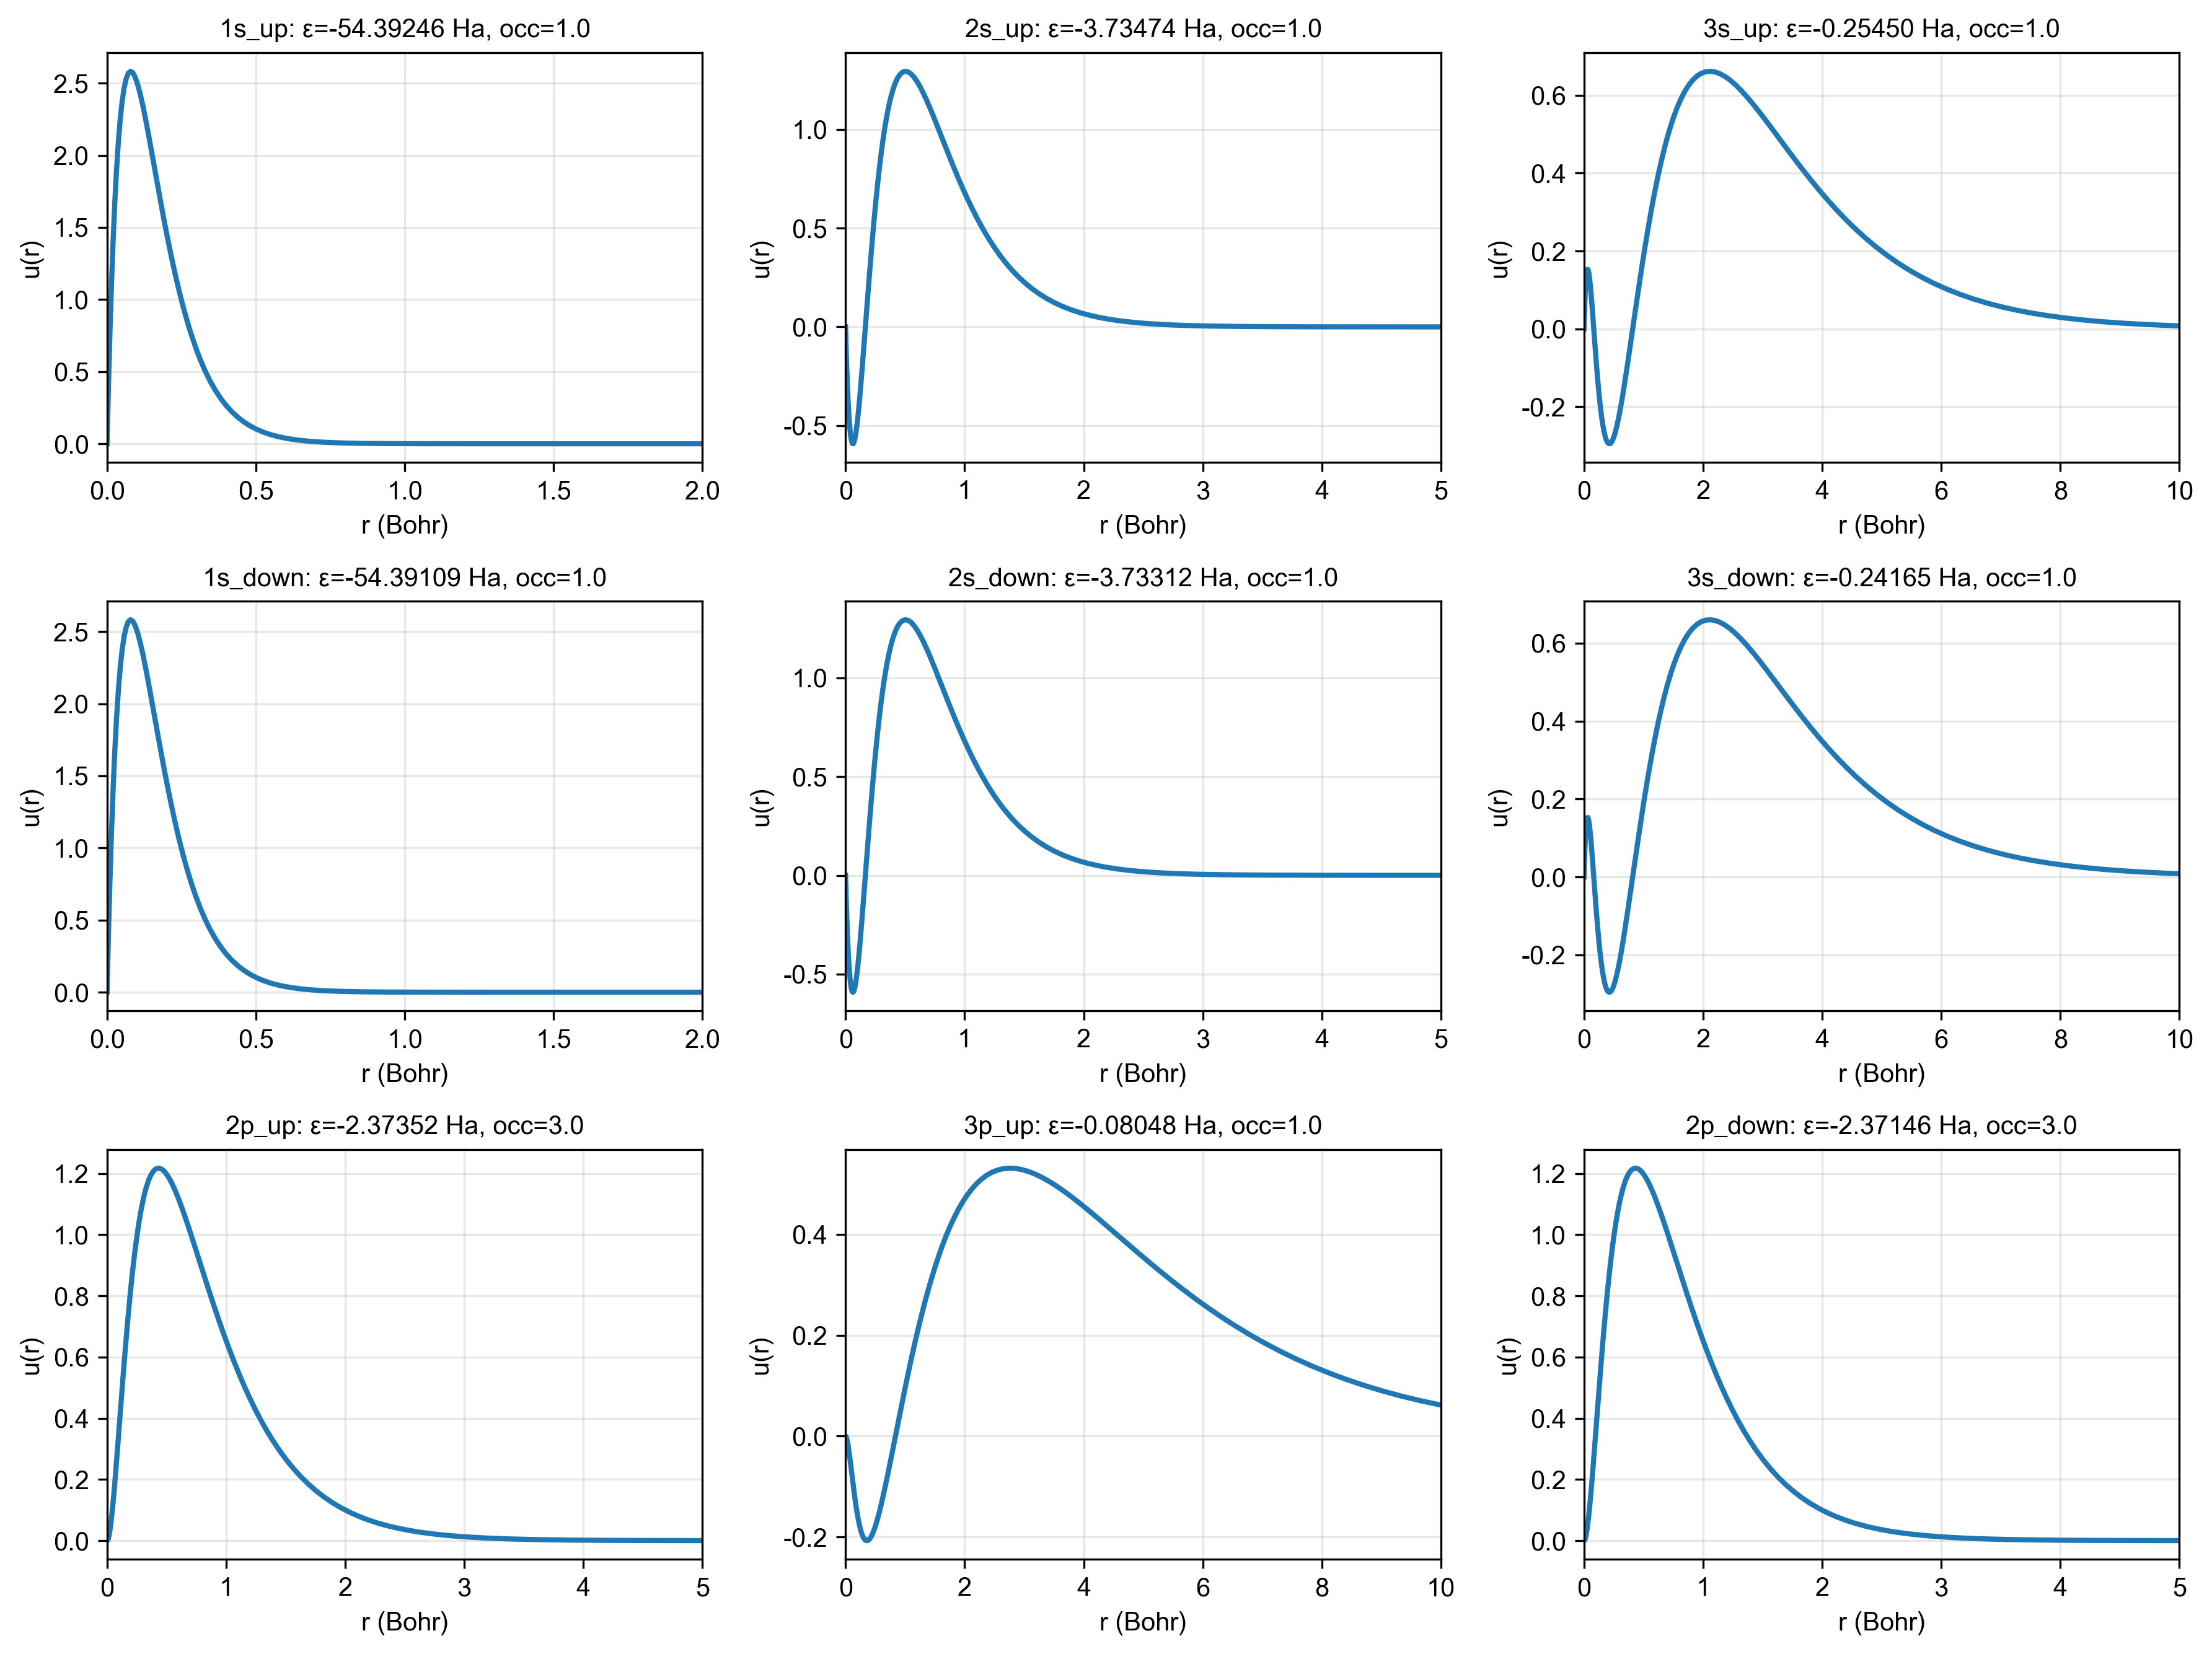
\includegraphics[width=0.8\textwidth]{figures/Al_lsda.png}
    \caption{铝原子占据态波函数}
\end{figure}

\section{误差分析与讨论}

\subsection{精度分析}

从与 NIST LSD 参考数据对比可以看出:
\begin{enumerate}
    \item \textbf{总能量误差}:重原子更精确(Al: 1.6\%,C: 2.6\%,Li: 4.4\%,He: 6.4\%,H: 10.9\%)
    \item \textbf{内层轨道}(1s):误差较小(1.4-15.1\%)
    \item \textbf{外层轨道}(2p, 2s):误差较大(13-41\%)
\end{enumerate}

\subsection{误差来源}

\subsubsection{自相互作用误差(SIE)}

氢原子只有一个电子,理论上不应有 Hartree 能和关联能。但 LSDA 计算中:
\begin{equation}
    E_H = \frac{1}{2}\int\int \frac{n(r)n(r')}{|r-r'|} dr dr' \neq 0
\end{equation}
这导致能级偏高(束缚变弱),总能量偏正。

\subsubsection{梯度修正缺失}

碳原子 2p 轨道密度梯度较大:
\begin{equation}
    s = \frac{|\nabla n|}{2k_F n} \quad \text{(约化梯度)}
\end{equation}
其中 $k_F = (3\pi^2 n)^{1/3}$ 为费米波矢。LDA 假设局域均匀性($s \to 0$),在高梯度区域失效。

\subsubsection{长程关联}

原子外层轨道(如 2p)在远离核区域($r \to \infty$)呈指数衰减。LDA 基于均匀电子气,无法正确描述长程行为。

\subsubsection{数值验证}

通过以下测试排除了数值方法误差:
\begin{enumerate}
    \item \textbf{网格收敛性}:Richardson 外推表明,网格细化对 C 2p 能级改善 $<0.01\%$
    \item \textbf{边界条件}:Shooting 打靶法细化能量,改善 $<0.01\%$
    \item \textbf{积分精度}:梯形积分与高阶 Gauss 求积差异 $<10^{-5}$ Ha
\end{enumerate}

因此,误差主要来源于 LSDA 泛函本身的物理近似,而非数值实现。NIST 参考数据也使用 LSD,但数值实现细节可能不同。

\subsection{重原子趋势}

重原子精度更高的原因:
\begin{enumerate}
    \item 电子密度更高,更接近均匀电子气假设
    \item SIE 的相对贡献随电子数增加而减小
    \item 内层轨道屏蔽效应使计算更稳定
\end{enumerate}

\section{总结}

本工作实现了原子的 Hartree-Fock 和 LSDA-DFT 自洽场计算程序,主要成果包括:

\begin{enumerate}
    \item \textbf{理论方法}:
          \begin{itemize}
              \item 自旋极化 HF:精确交换(Slater 积分 + Wigner-3j)
              \item 自旋极化 LSDA:Dirac 交换 + VWN 关联
              \item SCF 迭代:密度混合收敛
          \end{itemize}

    \item \textbf{数值方法}:
          \begin{itemize}
              \item 指数变换网格:近核密、远场疏
              \item 变量变换:消除一阶导数项,精度提升
              \item 梯形积分:两段累积法高效计算
          \end{itemize}

    \item \textbf{计算结果}:
          \begin{itemize}
              \item 测试了 H, He, Li, C, Al 共5个原子
              \item 给出所有占据态和第一个未占据态能级
              \item 导出波函数(径向采样 201 点)
          \end{itemize}

    \item \textbf{误差分析}:
          \begin{itemize}
              \item 主要误差来源:SIE + 梯度修正缺失 + 长程关联
              \item 数值方法误差 $<0.01\%$(已验证)
              \item 重原子精度更高(Al 误差 1.6\%)
          \end{itemize}
\end{enumerate}

完整结果保存在 \texttt{test\_results/}(JSON 数据)和 \texttt{figures/}(波函数图)目录。

\section*{参考文献}

\begin{enumerate}
    \item Vosko, S. H., Wilk, L., \& Nusair, M. (1980). Accurate spin-dependent electron liquid correlation energies. \textit{Can. J. Phys.}, 58(8), 1200-1211.
    \item Perdew, J. P., \& Zunger, A. (1981). Self-interaction correction to DFT. \textit{Phys. Rev. B}, 23(10), 5048.
    \item Slater, J. C. (1960). \textit{Quantum theory of atomic structure}. McGraw-Hill.
    \item Martin, R. M. (2004). \textit{Electronic structure: basic theory and practical methods}. Cambridge Univ. Press.
    \item NIST Atomic Reference Data: \href{https://www.nist.gov/pml/atomic-reference-data-electronic-structure-calculations}{nist.gov/pml/atomic-reference-data}
    \item Certik, O. et al. DFTatom: \href{https://github.com/certik/dftatom}{github.com/certik/dftatom}
    \item Adrian, R. DFT for an Atom: \href{https://compphys.go.ro/dft-for-an-atom/}{compphys.go.ro/dft-for-an-atom}
\end{enumerate}

\end{document}
